\documentclass[12pt,a4paper,spanish]{article}
\usepackage[utf8]{inputenc}
\usepackage[T1]{fontenc}
\usepackage[spanish]{babel}
\usepackage{graphicx}
\usepackage[colorlinks=true,linkcolor=black,urlcolor=black]{hyperref}
\usepackage{float}
\usepackage{amsmath}
\usepackage[margin=2.5cm]{geometry}
\usepackage{tocbibind}
\usepackage{titlesec}

% Configuración de los títulos de sección
\titleformat{\section}
  {\normalfont\Large\bfseries}{\thesection}{1em}{}
\titleformat{\subsection}
  {\normalfont\large\bfseries}{\thesubsection}{1em}{}

\begin{document}
% Portada
\begin{titlepage}
    \centering
    \vspace*{1cm}
    
\includegraphics[width=0.8\linewidth]{espe.png}\\[0.5cm]
    
    \Large \textbf{Departamento de Ciencias de la Computación}\\
    \large \textbf{Universidad de las Fuerzas Armadas - ESPE}\\[0.5cm]
    
    \Huge \textbf{Resumen de Películas}\\[0.3cm]
    \Large \textbf{Parcial No. 1}\\[0.8cm]
    
    \textbf{Nombres:}\\
    Yeshua Amador Chiliquinga Amaya\\[0.3cm]
    
    \textbf{Carrera / Asignatura:} Ingeniería de Software / Ingeniería de Seguridad de Software\\
    \textbf{NRC:} 2540\\
    \textbf{Nombre del profesor:} Walter Fuertes, PhD\\[0.5cm]
    
    \textbf{Fecha de presentación:} 24 de mayo del 2025\\[1cm]    
    \vfill
\end{titlepage}
% Índice de contenido

\tableofcontents
\thispagestyle{empty} % Elimina el número de página en el índice
\newpage
\setcounter{page}{1} % Reinicia el contador de páginas después del índice

\section{Resúmenes de Películas}
\addcontentsline{toc}{section}{Resúmenes de Películas}

\subsection{El Código Enigma (The Imitation Game, 2014)}
\begin{figure}[H]
    \centering
    
\includegraphics[width=0.8\textwidth]{codigo_enigma.png}
    \caption{El Código Enigma (2014)}
    \label{fig:codigo_enigma}
\end{figure}

\textbf{Director:} Morten Tyldum\\
\textbf{Reparto principal:} Benedict Cumberbatch, Keira Knightley, Matthew Goode\\
\textbf{Reflexión:} \emph{El Código Enigma} es un poderoso recordatorio de cómo las mentes más brillantes a menudo se esconden detrás de las apariencias más inesperadas. La historia de Alan Turing me conmovió profundamente, mostrándome que el genio puede florecer incluso en las circunstancias más adversas. Lo que más me impacta es cómo su legado en la informática moderna y la inteligencia artificial fue opacado por la intolerancia de su época.\\

\textbf{Lección:} Esta película me enseñó que las ideas verdaderamente revolucionarias a menudo enfrentan resistencia, pero que el valor de la verdad y la innovación trasciende el tiempo. Me motiva a valorar mi propia singularidad y a nunca subestimar el poder de pensar diferente, incluso cuando el mundo parece estar en tu contra.

\vspace{1cm}

\subsection{Una Mente Brillante (A Beautiful Mind, 2001)}
\begin{figure}[H]
    \centering
    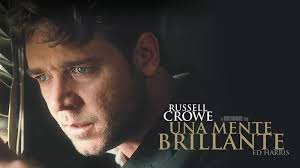
\includegraphics[width=0.8\textwidth]{una_mente_brillante.jpg}
    \caption{Una Mente Brillante (2001)}
    \label{fig:una_mente_brillante}
\end{figure}

\textbf{Director:} Ron Howard\\
\textbf{Reparto principal:} Russell Crowe, Ed Harris, Jennifer Connelly\\
\textbf{Reflexión:} \emph{Una Mente Brillante} es un viaje conmovedor a través de la mente de un genio atormentado. La interpretación de Russell Crowe como John Nash me hizo reflexionar sobre la delgada línea entre la locura y la genialidad. Lo que más me conmovió fue la relación de Nash con su esposa Alicia, mostrando que el amor incondicional puede ser el ancla que necesitamos en nuestros momentos más oscuros.\\

\textbf{Lección:} Esta película me enseñó que nuestras mayores batallas a menudo son internas, y que la verdadera grandeza no está en ser perfecto, sino en aprender a vivir con nuestras imperfecciones. Me inspira a ser más compasivo conmigo mismo y con los demás, recordando que todos luchamos batallas que los demás no pueden ver.

\vspace{1cm}

\subsection{Mente Indomable (Good Will Hunting, 1997)}
\begin{figure}[H]
    \centering
    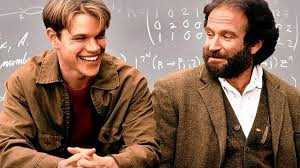
\includegraphics[width=0.8\textwidth]{mente_indomable.jpg}
    \caption{Mente Indomable (1997)}
    \label{fig:mente_indomable}
\end{figure}

\textbf{Director:} Gus Van Sant\\
\textbf{Reparto principal:} Matt Damon, Robin Williams, Ben Affleck, Minnie Driver\\
\textbf{Reflexión:} \emph{Mente Indomable} es un recordatorio poderoso de que el mayor obstáculo para nuestro éxito a menudo somos nosotros mismos. La interpretación de Robin Williams como el terapeuta Sean Maguire me dejó sin aliento, especialmente en esa escena del parque donde le dice a Will: "No es tu culpa". Es increíble cómo una película puede mostrarte que la inteligencia académica es solo una parte de lo que nos hace humanos.\\

\textbf{Lección:} Lo que más me impactó fue ver a Will darse cuenta de que su verdadera libertad no estaba en escapar de su pasado, sino en enfrentarlo. Esta película me motiva a no dejar que mis miedos y heridas del pasado definan mi futuro, y a recordar que todos merecemos amor y oportunidades, sin importar de dónde venimos.

\end{document}

